Aunque la exportación a Emscripten puede considerarse parte del proceso de implementación, su extensión e importancia en este documento hace que valga la pena dedicarle su propio capítulo.

Uno de los puntos fuertes de nuestro planner es el poder ejecutarlo en web. El hecho de estar programado en C++, sin embargo, dificulta esta tarea. Teniendo cuenta una serie de consideraciones, es posible adaptar código C++ a web a través de Emscripten.

\label{emscripten}
\section{Consideraciones previas}
En esta sección se describen diversas consideraciones que se han tenido en cuenta a la hora de adaptar el código con Emscripten.

%%%%%%%%%%%%%%%%%%%%%%%%%%%%%%%%%%%%%%%%%%%%%%%%%%%%%%%%%%%%%%%%%%%%%%%%%%%%%
%%%%%%%%%%%%%%%%%%%%%%%%%%%%%%%%%%%%%%%%%%%%%%%%%%%%%%%%%%%%%%%%%%%%%%%%%%%%%
%%%%%%%%%%%%%%%%%%%%%%%%%%%%%%%%%%%%%%%%%%%%%%%%%%%%%%%%%%%%%%%%%%%%%%%%%%%%%

\subsection{Sobre Emscripten}
\label{about_emscripten}
Emscripten es capaz de compilar código IL (Intermediate Language) a Javascript. IL es un lenguaje de código máquina que se puede generar compilando desde otros lenguajes, entre ellos C++ usando el compilador LLVM. Dado que Emscripten compila desde IL (y no C++ directamente) realmente esto significa que podemos ejecutar código escrito en diversos lenguajes a través de Emscripten.

Emscripten\footfullcite{kripken_cppcon} nació como respuesta a la necesidad de escribir programas para web en lenguajes tradicionales de escritorio, con el objetivo de ganar velocidad, trabajar con un lenguaje familiar, y aprovechar las librerías existentes en dichos lenguajes. Hasta su aparición la única alternativa para poder hacer esto era el uso de plugins embebidos en el navegador, lo cual fracasó debido a la falta de estandarización y a la evolución de los propios navegadores, que cada vez más rechazan los plugins desde la popularización de las plataformas móviles.

Dada la extensión de funcionalidades de Javascript, para realizar el compilado se ha utilizado un subset de este, ``asm.js". Asm.js es un lenguaje intermedio que podemos ejecutar en navegadores; tiene una serie de restricciones con respecto a Javascript, como por ejemplo el hecho de ser un lenguaje tipado (aunque Javascript no lo es, en asm.js se comprueba el tipo de cada variable antes de trabajar con ella) o el requerimiento de trabajar sobre una única pila de memoria (un simple array de Javascript dentro del cual deben estar todos los datos que utilice el programa).

Si se aplica esta filosofía al código que programamos en C++, se puede entender fácilmente que dicha pila de memoria equivale a la memoria tal y como la ve un programa tradicional en C++. Es posible reservar memoria dentro de esta pila, y tener punteros a posiciones de la pila (que en realidad no son más que simples índices). Tiene un funcionamiento similar al Memory Pool descrito en el apartado \ref{engine_memory}.

Aunque en cuanto a eficiencia el código en asm.js en web está en torno al 50-67\% de su equivalente en escritorio, los resultados pueden ser sorprendentes pues asm.js es capaz de superar en velocidad a su equivalente escrito en Javascript tradicional. Al trabajar sobre datos estáticos y memoria pre-inicializada, el código resultante cuenta con una serie de optimizaciones que un programador no suele realizar manualmente.

Una de las actuales tendencias del web es la ejecución de código máquina, para lo cual está en fase de desarrollo la tecnología ``WebAssembly". Sin embargo, aún a día de hoy no está del todo claro cuando estará lista lo suficientemente avanzada\footfullcite{emscripten_ready}, por lo que el papel de asm.js es importante como paso intermedio, para que los desarrolladores puedan ir adoptando la tecnología antes de ser funcional del todo. Emscripten también tiene un rol muy importante en este proceso, porque es el encargado tanto de compilar a asm.js hoy como lo será de compilar a WebAssembly en el futuro\footfullcite{webasm_roadmap}.

Emscripten ya se está utilizando hoy en día en diversos proyectos de cierta categoría, especialmente en aplicaciones gráficas.

Es importante también tener en cuenta algunos de los defectos de utilizar Emscripten respecto a programar directamente en Javascript:

\begin{itemize}
    \item Es necesario saber desde el primer momento cuanta memoria se va a necesitar. Aunque superar dicha memoria no hará que el programa falle (Emscripten es capaz de reasignar memoria cuando se sobrepasa el límite), permitir que esto ocurra no es en absoluto recomendable, puesto que ralentizaría el programa.
    
    \item Se requiere un proceso de adaptación considerable: muchas de las cosas que el programador da por sentadas en C++ no se cumplen en Javascript. Como se puede ver a lo largo del capítulo \ref{emscripten}, no se puede inicializar el programa, gestionar los ficheros o ejecutar el bucle del programa del mismo modo en que se haría en C++.
    
    \item Se pierde poder de decisión sobre algunas de las tecnologías que se pueden querer utilizar porque simplemente no están disponibles, como versiones modernas de OpenGL o las operaciones SIMD (un tipo de operaciones que permite realizar cálculos con múltiples datos en una sola instrucción\footfullcite{simd}). Esto cambiará en el futuro según avance la tecnología, pero a día de hoy es un limitante.
    
    \item Si se desea que el mismo código se pueda ejecutar en diversas plataformas, habrá otro proceso de adaptación considerable para hacer que el programa tenga en cuenta las consideraciones mencionadas según la plataforma. En realidad esto es más bien un defecto de la programación multi-plataforma que de Emscripten, pero se debe tener en cuenta que existirá un esfuerzo extra de desarrollo y un aumento de la complejidad del código.
    
    \item El debugging resulta sensiblemente más incómodo que con Javascript o C++ en escritorio\footfullcite{emscripten_debugging}. Normalmente para seguir los errores se hace uso de impresiones a través de la consola y el stack-trace que devuelve Emscripten cuando se produce un error (el cual no siempre es suficientemente descriptivo).
\end{itemize}

%%%%%%%%%%%%%%%%%%%%%%%%%%%%%%%%%%%%%%%%%%%%%%%%%%%%%%%%%%%%%%%%%%%%%%%%%%%%%
%%%%%%%%%%%%%%%%%%%%%%%%%%%%%%%%%%%%%%%%%%%%%%%%%%%%%%%%%%%%%%%%%%%%%%%%%%%%%
%%%%%%%%%%%%%%%%%%%%%%%%%%%%%%%%%%%%%%%%%%%%%%%%%%%%%%%%%%%%%%%%%%%%%%%%%%%%%

\subsection{API gráfica}
\label{emscripten_gapi}
Como se ha podido ver en el apartado \ref{APIS}, el motor está pensado para funcionar utilizando la API gráfica Vulkan. El primer paso para hacer funcionar el programa con Emscripten ha sido utilizar una API gráfica que sea compatible con las tecnologías web.

WebGL está basado en OpenGL ES 2, y Emscripten puede reconocer las llamadas a esta segunda API y transformarlas en llamadas a WebGL. De modo que para hacer funcionar el motor será necesario con buscar los puntos donde se interactúe con la API de Vulkan y cambiarlos para que funcionen con OpenGL ES 2.

En el momento de realizar la exportación se deberá tener en cuenta que Vulkan y WebGL son completamente incompatibles. En el fondo no se sustituyen directamente las llamadas a la API de Vulkan, sino que se detectan los puntos en que un conjunto de código se puede considerar equivalente a una llamada de OpenGL. El código de Vulkan es mucho más complejo y largo de lo que requiere OpenGL, y lo que en Vulkan requiere muchas líneas de código puede hacerse en OpenGL con una sola llamada.

También será necesario adaptar los shaders y el proceso de carga de estos, dado que OpenGL ES 2 tiene limitaciones como la necesidad de definir el número de variables que recibirá el shader antes de compilarlo, dificultando la carga dinámica de luces. Aunque ambas APIs utilizan el mismo lenguaje de shading, GLSL, no es posible reutilizar sin más el código porque se utilizan diferentes versiones de este. En WebGL se utiliza la versión 100 de GLSL mientras que SPIR-V (véase \ref{shaders}) parte de la versión 450; se trata de versiones muy diferentes y aunque se han reutilizado algunos fragmentos, no es posible reaprovechar el código por completo.

%%%%%%%%%%%%%%%%%%%%%%%%%%%%%%%%%%%%%%%%%%%%%%%%%%%%%%%%%%%%%%%%%%%%%%%%%%%%%
%%%%%%%%%%%%%%%%%%%%%%%%%%%%%%%%%%%%%%%%%%%%%%%%%%%%%%%%%%%%%%%%%%%%%%%%%%%%%
%%%%%%%%%%%%%%%%%%%%%%%%%%%%%%%%%%%%%%%%%%%%%%%%%%%%%%%%%%%%%%%%%%%%%%%%%%%%%

\subsection{Comunicación C++/Javascript}
\label{emscripten_comm}
Como es de esperar, es posible (necesario, de hecho) comunicar el código de Javascript con el código compilado desde C++\footfullcite{kripken_interacting}. En el desarrollo de la aplicación en C++ pueden definirse funciones pensadas para ser llamadas desde Javascript, y en el momento de compilar deben especificarse cuáles son esas funciones. Posteriormente, el Javascript resultante al compilar pone a disposición del desarrollador las funciones \texttt{cwrap} i \texttt{ccall}.

La función \texttt{cwrap} provee una función intermedia que se puede llamar como si de una función normal de Javascript se tratara. Esta función se encargará de llamar a su vez a la función de C++ correspondiente. En cambio, \texttt{ccall} permite llamar directamente a la función de C++, pero como se explica a continuación es más verboso, por lo que si la función va a ser llamada varias veces puede ser más recomendable utilizar la primera alternativa.

Ambas opciones requieren que se especifique la firma de las funciones que van a ser llamadas. La firma de una función define el tipo de los parámetros que recibe y el tipo del valor de devuelve. De ahí que se diga que \texttt{ccall} es más verboso: cada vez que se llame es necesario especificar la firma mientras que con \texttt{cwrap} solo se debe hacer una vez.

Otro detalle importante a tener en cuenta es que no cualquier función puede ser llamada desde Javascript. Emscripten sólo permite que llamemos a funciones propias del lenguaje C, dado que C++ altera el nombre de las funciones al compilarlas (C++ permite a dos funciones llamarse igual si tienen firmas distintas, pero lo resuelve cambiando los nombres en el compilado resultante). Para garantizar que las funciones sean propias de C cuando programamos en C++ se utiliza el prefijo \texttt{extern "C"} antes de la definición.

Como se verá en el apartado \ref{init_emscripten} la comunicación entre C++ y Javascript es importante para controlar el flujo de la aplicación, pero también lo será para que desde el lado web se puedan crear interacciones que tengan efecto en el planificador. Con HTML y Javascript se pueden crear toda clase de eventos que pueden transmitirse a C++, como elementos de interfaz. Además, el planificador no controla los datos relacionados con el dominio de la aplicación, como por ejemplo qué muebles están disponibles en qué países; esta información se transmitirá a la aplicación a través de la web.

%%%%%%%%%%%%%%%%%%%%%%%%%%%%%%%%%%%%%%%%%%%%%%%%%%%%%%%%%%%%%%%%%%%%%%%%%%%%%
%%%%%%%%%%%%%%%%%%%%%%%%%%%%%%%%%%%%%%%%%%%%%%%%%%%%%%%%%%%%%%%%%%%%%%%%%%%%%
%%%%%%%%%%%%%%%%%%%%%%%%%%%%%%%%%%%%%%%%%%%%%%%%%%%%%%%%%%%%%%%%%%%%%%%%%%%%%

\subsection{Inicialización y bucle de ejecución}
\label{init_emscripten}
Uno de los inconvenientes de Emscripten es que Javascript ejecuta todos los procesos relacionados con la página en un único hilo de ejecución, incluyendo el renderizado, la gestión de eventos y la actualización de la propia página.

Javascript tiene una naturaleza orientada a eventos\footfullcite{javascript_queue}: dispone de una cola de eventos que se van añadiendo y ejecutando en un orden difícil de predecir. Entre esos eventos estará la propia ejecución del código Javascript y en consecuencia el código generado con Emscripten, pero también el resto de eventos mencionados que gestionan el comportamiento de la página. Si uno de los eventos tarda demasiado en terminar, bloqueará la cola de eventos y provocará que toda la página se bloquee.

Como el desarrollador no sabe en que orden se ejecutan los eventos, se dice que el lenguaje es asíncrono, y eso implica que se debe programar con cuidado para controlar que todo ocurra en el orden que se espera. La naturaleza asíncrona de Javascript puede confundir al programador haciéndole pensar que puede utilizar más de un hilo de ejecución (dado que en otros lenguajes la programación multi-hilo y la asincronía están estrechamente relacionadas); es importante tener presente que no es posible realizar dos tareas al mismo tiempo en este lenguaje. Sí se espera, en cambio, que WebAssembly pueda en el futuro ejecutar programas multi-hilo.

Como se menciona en el apartado \ref{emscripten_comm}, el flujo de la aplicación debe controlarse desde Javascript. El bucle de ejecución (\ref{fps_bucle_ejecucion}) es un bucle infinito, por lo que si lo ejecutamos estando dentro de C++ bloquearemos por completo la aplicación impidiendo que la cola avance. Por lo tanto el primer paso para hacer funcionar la aplicación pasa por hacer que las funciones \texttt{Update} y \texttt{Draw} del motor se llamen desde Javascript.

Para conseguirlo se debe utilizar la función \texttt{setInterval}\footfullcite{setInterval}, que dado un intervalo de tiempo añade un evento para llamar a una función repetidamente. Especificando un intervalo de $1/6$ segundos, podemos hacer que la función de \texttt{Update} se llame 60 veces por segundo. Es importante tener en cuenta que setInterval no garantiza que la función se llame realmente en el intervalo dado, sino que ese el mínimo de tiempo que se tardará en llamar; si la aplicación se ralentiza Javascript esperará a que termine la repetición anterior para llamar de nuevo. También el cálculo del tiempo entre frames (explicado en el apartado \ref{fps_bucle_ejecucion}) se hará desde Javascript aunque esto no es estrictamente necesario.

Antes de iniciar el bucle de ejecución se llamará a una función \texttt{Init}, con el objetivo de incializar el motor y el contexto de WebGL.

%%%%%%%%%%%%%%%%%%%%%%%%%%%%%%%%%%%%%%%%%%%%%%%%%%%%%%%%%%%%%%%%%%%%%%%%%%%%%
%%%%%%%%%%%%%%%%%%%%%%%%%%%%%%%%%%%%%%%%%%%%%%%%%%%%%%%%%%%%%%%%%%%%%%%%%%%%%
%%%%%%%%%%%%%%%%%%%%%%%%%%%%%%%%%%%%%%%%%%%%%%%%%%%%%%%%%%%%%%%%%%%%%%%%%%%%%

\subsection{Gestión de ficheros}
\label{emscripten_filesistem}
A lo largo de la ejecución del planificador será necesario proveer al software con una serie de assets (modelos 3D o texturas) y datos que provienen de ficheros. En C y C++ típicamente se accede al sistema de ficheros a través de la función \texttt{fopen}, que solicita al sistema operativo acceso a un fichero determinado; y después se extrae la información de este.

En C++, los datos del fichero que se quiere leer pasan a estar disponibles justo en el momento en que se piden, de forma síncrona; pero el proceso es mucho más complicado en Javascript. En Javascript no tenemos un sistema de ficheros, y si queremos tener acceso a alguno, debemos antes solicitarlo a un servidor remoto.

Es un problema porque las peticiones a servidores remotos se hacen de forma asíncrona (técnicamente se puede hacer de forma síncrona, pero se trata de una función obsoleta, que debe ser evitada y que tiene efectos secundarios como el bloqueo de la página); el hecho de que el funcionamiento sea diferente según la plataforma dificulta considerablemente el desarrollo.

Emscripten pone a disposición de los desarrolladores varias soluciones para facilitar el acceso a ficheros externos\footfullcite{emscripten_files}. Para que los cambios a realizar según la plataforma sean mínimos, Emscripten emula un sistema de ficheros de modo que podamos utilizarlo con \texttt{fopen} igual que lo haríamos en C++. El modo en que esos ficheros pasen a estar disponibles en el sistema de ficheros, en cambio, puede variar:

\begin{itemize}
    \item Precarga sistema de ficheros: Los ficheros que se pre-carguen con este sistema, en el momento de compilar, se añadirán a un único archivo binario que se descarga al navegador junto al código generado. El sistema de archivos de Emscripten tiene una lista de estos ficheros con sus rutas y su posición en el archivo de precarga. Teniendo en cuenta que tanto los modelos 3D como las texturas son bastante pesados, y que en un planificador puede haber una gran cantidad, esto aumentaría considerablemente el peso de la descarga inicial, y el tiempo de carga; pero la ventaja es que los archivos pasan a estar disponibles de manera síncrona y sin cambiar en absoluto el código que los lee.
    
    \item Descarga síncrona: Emscripten provee la función \texttt{emscripten\_wget}, que dada la url de un archivo la descarga de forma síncrona a través del navegador. También se necesita dar un nombre al archivo cargado puesto que Emscripten lo guarda en el sistema de archivos virtual para que podamos acceder a él con \texttt{fopen}. Aunque con este método no sería necesario cambiar el flujo de la ejecución, como ya se ha mencionado este sistema es obsoleto.
    
    \item Descarga asíncrona: La alternativa asíncrona al anterior método es \texttt{emscripten\_async\_wget}. Del mismo modo que antes, esta función carga el archivo solicitado en el sistema de ficheros virtual, pero si intentamos leerlo justo después de llamar a la función la carga fallará, puesto que la carga aún no se ha realizado realmente. Para acceder al archivo debemos utilizar un puntero de función (o callback) que pasamos como parámetro a \texttt{emscripten\_wget\_async}, y que se llamará si el archivo se carga correctamente. También debemos pasarle otro callback que se llamará en caso de que la descarga fracase, y que nos permite gestionar tal evento. El callback de carga también recibe como parámetro los datos binarios del fichero solicitado, de modo que aunque seguimos pudiendo acceder a él desde el sistema de ficheros virtual con \texttt{fopen}, no es realmente necesario. Este sistema nos obliga a cambiar el flujo del programa, puesto que al no disponer aún del fichero solicitado, no podemos hacer nada que haga uso de este hasta que el callback de éxito se haya llamado.
\end{itemize}

La segunda opción ni siquiera será tenida en cuenta por sus características. Por un lado la primera alternativa obliga a descargar todos los assets desde el principio, y por otro la última no da acceso inmediato a los archivos como se suele presuponer cuando se programa en C++.

La solución pasa por utilizar una mezcla de ambas. Cuando se carga un modelo 3D o una textura, por la fuerza es necesario tener una respuesta inmediata, pero una vez se ha cargado un asset y se está utilizando, nada impide cambiar en un momento dado cambiar los datos de ese asset con un contenido diferente. Para tener acceso inmediato a los assets se pre-cargargan unos assets ``dummies", muy pequeños, que no supone ningún coste añadir junto con la carga de la app.

Cuando se quiera tener acceso a un asset, este se solicitará de forma asíncrona, pero inmediatamente después se proveerá al motor con un dummy, y se guardará el identificador para tener acceso al asset guardado. En el momento en que la carga asíncrona finalice, el asset dummy será sustituido por el correcto. Durante el tiempo intermedio se verá en pantalla un asset que no es el que debería verse, pero se trata de un tiempo generalmente muy corto y da un efecto de ``carga" al que los usuarios ya están bastante habituados.

%%%%%%%%%%%%%%%%%%%%%%%%%%%%%%%%%%%%%%%%%%%%%%%%%%%%%%%%%%%%%%%%%%%%%%%%%%%%%
%%%%%%%%%%%%%%%%%%%%%%%%%%%%%%%%%%%%%%%%%%%%%%%%%%%%%%%%%%%%%%%%%%%%%%%%%%%%%
%%%%%%%%%%%%%%%%%%%%%%%%%%%%%%%%%%%%%%%%%%%%%%%%%%%%%%%%%%%%%%%%%%%%%%%%%%%%%

\section{Pasos para la exportación}
Una vez descritas las consideraciones a tener en cuenta para poder realizar la exportación, se va a proceder a exportar el código. En esta sección se describirá el proceso paso a paso. 

%%%%%%%%%%%%%%%%%%%%%%%%%%%%%%%%%%%%%%%%%%%%%%%%%%%%%%%%%%%%%%%%%%%%%%%%%%%%%
%%%%%%%%%%%%%%%%%%%%%%%%%%%%%%%%%%%%%%%%%%%%%%%%%%%%%%%%%%%%%%%%%%%%%%%%%%%%%
%%%%%%%%%%%%%%%%%%%%%%%%%%%%%%%%%%%%%%%%%%%%%%%%%%%%%%%%%%%%%%%%%%%%%%%%%%%%%

\subsection{Gestión del código discordante}
\label{cpp_macros_for_platforms}
En C++, las discordancias entre las distintas plataformas se resuelve mediante macros. Una macro es un fragmento de código que se ejecuta antes de la compilación, y es capaza de modificar el código en función de diversos factores. 

Normalmente, el código que es específico para una plataforma provoca un fallo en el resto de plataformas, por lo que se requiere ``intercambiar" estos fragmentos de código incompatibles. También las librerías a utilizar pueden cambiar y la firma de algunas funciones.

Cuando compilamos con Emscripten, se define la macro \texttt{\_\_EMSCRIPTEN\_\_}, permitiéndonos controlar fácilmente el código que se compilará en cada plataforma.

Un modo de entender lo que hacen las macros en C++ es imaginar que literalmente modifican el código. Desde el punto de vista del código generado, el uso de macros es equivalente a borrar y añadir la parte correspondiente a una u otra plataforma. Los distintos tipos de macros son simplemente formas diferentes de realizar modificaciones al código en tiempo de compilación.

\begin{lstlisting}
#ifdef __EMSCRIPTEN__
    // Codigo especifico para Emscripten
#endif

#ifndef __EMSCRIPTEN__
    // Codigo que debe ignorarse al compilar con Emscripten
#endif
\end{lstlisting}

También es necesario en determinadas ocasiones utilizar funciones distintas para realizar la misma operación en diferentes plataformas. Sería posible solucionar este caso mediante la macro \texttt{\#ifdef}, pero tendría que hacerse cada vez que se utiliza dicha función.

Las macros de definición de C++ permiten incluir parámetros; por ejemplo la macro \texttt{\#define f(A) A * 2} cogería el parámetro ``A" y lo multiplicaría por dos. Lo interesante es que el usar las macros de este modo no requiere que ``A" tenga ningún tipo en especial, ni siquiera que sea una variable; siempre y cuando el código resultante al procesar la macro sea válido.

Esta característica se utiliza, por ejemplo, con la función \texttt{fopen}. En Windows se requiere utilizar la función \texttt{fopen\_s}, que tiene una firma distinta que \texttt{fopen}; mientras que en Emscripten solo se reconoce esta última, provocando un fallo de compilación si se utiliza \texttt{fopen\_s}. Se puede solucionar esto con la macro:

\begin{lstlisting}
#ifdef __EMSCRIPTEN__
#define fopen_s(pFile,filename,mode) ((*(pFile))=fopen((filename),(mode)))==NULL
#endif
\end{lstlisting}

Definiendo esto podemos utilizar \texttt{fopen\_s} con normalidad sin tener que preocuparnos por la plataforma dado que, sólo en Emscripten, cuando el compilador se encuentre una llamada a \texttt{fopen\_s} la sustituirá por su equivalente.

Aunque las macros pueden resultar tentadoras, es buena costumbre no abusar de ellas, dado que pueden terminar generando un código extremadamente confuso y difícil de mantener. Es por ello que durante todo el desarrollo siempre se ha exigido tener una buena razón antes de utilizarlas, especialmente en niveles más altos de complejidad como en este último ejemplo.

%%%%%%%%%%%%%%%%%%%%%%%%%%%%%%%%%%%%%%%%%%%%%%%%%%%%%%%%%%%%%%%%%%%%%%%%%%%%%
%%%%%%%%%%%%%%%%%%%%%%%%%%%%%%%%%%%%%%%%%%%%%%%%%%%%%%%%%%%%%%%%%%%%%%%%%%%%%
%%%%%%%%%%%%%%%%%%%%%%%%%%%%%%%%%%%%%%%%%%%%%%%%%%%%%%%%%%%%%%%%%%%%%%%%%%%%%

\subsection{Compilación}
Normalmente se compila a Emscripten mediante la terminal de comandos. Se debe conocer en cierta profundidad las opciones de compilado, por lo que en este apartado se introduce el proceso de compilación y algunas de las opciones más genéricas. En los próximos apartados se comentarán otras opciones más específicas.

Tras la instalación del SDK de Emscripten, se dispone el comando \texttt{emcc}\footfullcite{emscripten_build_projects}. En su forma más básica, este comando puede utilizarse especificando los ficheros C++ de input y el fichero Javascript de output con la opción \texttt{-o}: \texttt{emcc codigo.cpp -o resultado.js}. En la práctica, será necesario aplicar diversas opciones para hacer que un código complejo funcione.

A continuación se describen los que se han utilizado para hacer funcionar el planificador:

\begin{itemize}
    \item \texttt{-s FULL\_ES2=1}: Activa la emulación de OpenGL ES 2. Sin esta opción no se traducen las llamadas de OpenGL a llamadas de WebGL.
    
    \item \texttt{-std=c++14}: Especifica la versión de C++ a compilar, en este caso C++14. Si se utilizan las características más nuevas del lenguaje, compilar con una versión más antigua puede provocar errores.
    
    \item \texttt{-msse} y \texttt{msse2}: Permite incorporar instrucciones SIMD SSE1 y SSE2. Las instrucciones SIMD permiten realizar cálculos con múltiples datos con una sola instrucción\footfullcite{simd} y no se profundizará sobre ellas en este documento. Son utilizadas por algunos componentes del motor para ganar eficiencia.
    
    \item \texttt{-s TOTAL\_MEMORY=N}, donde N es un número de bytes: Permite especificar la memoria que se le asigna al programa (véase la sección \ref{about_emscripten}). Dicha memoria será inicializada una sola vez al ejecutar el programa. Mediante la opción \texttt{-s ALLOW\_MEMORY\_GROWTH=1} se permite que en caso de superar el límite de memoria, esta se readapte, lo cual es extremadamente ineficiente pero puede ser útil para hacer debugging. Por defecto Emscripten asigna 16MB de memoria.
    
    \item \texttt{-s NO\_EXIT\_RUNTIME=1}: Hace que al finalizar la ejecución de la función \texttt{main} las funciones definidas desde C++ sigan estando disponibles para llamarse desde C++, y por extensión el resto de código disponible para ejecutarse.
    
    \item \texttt{-s EXPORTED\_FUNCTIONS="['\_f1','\_f2',...,'\_fn']"}: Define las funciones que están disponibles para ser llamadas desde Javascript. Para ello las funciones deben definirse con el prefijo \texttt{extern "C"}. Los nombres de las funciones van siempre con un caracter ``\_" antes.
    
    \item \texttt{-I path}, donde ``path" es la ruta de una carpeta o fichero: Define una carpeta o fichero de cabecera para que el compilador pueda encontrarlos. Esto incluye también las librerías externas.
    
    \item \texttt{--preload-file buildpath@runpath} donde buildpath es la ruta de un fichero o carpeta en el momento de compilar y runpath la ruta del mismo en tiempo de ejecución: Permite añadir ficheros estáticos al sistema de ficheros de Emscripten. Estos ficheros se pueden cargar de forma síncrona. Mediante el símbolo ``@" podemos definir un alias que será donde se ubicarán estos ficheros en el sistema de ficheros virtual.
\end{itemize}

%%%%%%%%%%%%%%%%%%%%%%%%%%%%%%%%%%%%%%%%%%%%%%%%%%%%%%%%%%%%%%%%%%%%%%%%%%%%%
%%%%%%%%%%%%%%%%%%%%%%%%%%%%%%%%%%%%%%%%%%%%%%%%%%%%%%%%%%%%%%%%%%%%%%%%%%%%%
%%%%%%%%%%%%%%%%%%%%%%%%%%%%%%%%%%%%%%%%%%%%%%%%%%%%%%%%%%%%%%%%%%%%%%%%%%%%%

\subsection{Exportación de la API gráfica}
Realizar un render en OpenGL resulta considerablemente más simple de lo que sería utilizando Vulkan. Utilizando las herramientas descritas en el apartado \ref{cpp_macros_for_platforms} es posible sustituir los fragmentos de código referentes a Vulkan por sus equivalentes en OpenGL ES 2.

Vulkan dispone de una serie de funciones de incialización. En su equivalente de OpenGL se aprovechan estas llamadas para incicializar OpenGL, compilar los shaders y obtener los identificadores de cada uno de los uniforms de este. También aquí se especifican todos los parámetros de OpenGL.

La escena del motor Manta, explicada en el apartado \ref{scene_hierarchy}, está gestionada por el espacio de nombre \texttt{SceneManager}. \texttt{SceneManager} se encarga de extraer los datos de la estructura de árbol en cada iteración, prepararlos, y ejecutar el renderizado. 

Al crear los componentes de malla de las distintas entidades que hay en la escena (explicados en el apartado \ref{mesh_light_cam}) es necesario cargar en memoria de GPU los datos de la malla (a no ser que esta haya sido cargada anteriormente, en cuyo caso se puede reutilizar). Ocurre igual con las texturas del material de la entidad. Al cargar estos elementos obtenemos un identificador para cada uno que debe guardarse y mantener relacionado con la entidad. 

Tanto este proceso como el propio renderizado se realiza dentro del propio \texttt{SceneManager}. El renderizado de cada entidad en OpenGL puede resumirse en los siguientes pasos:

\begin{itemize}
    \item Especificar el shader que va utilizarse para el renderizado, a través de un identificador que hemos obtenido al compilarlo.
    \item Transmitir a los drivers los datos de cada uniform, cuyos identificadores hemos guardado previamente, incluyendo los de la cámara, las luces, así como la transformación de la entidad.
    \item Especificar las texturas y datos que utiliza el material de la entidad y los distintos componentes de la malla por separado: vertices, uvs, colores, normales, tangentes, bitangentes e índices. Todos estos elementos ya están en memoria y solo es necesario especificar sus identificadores antes de renderizar.
    \item Mandar la orden de renderizado a OpenGL.
\end{itemize}

Todo este proceso se realiza mediante llamadas a la API de OpenGL ES 2 que, al compilar el código, Emscripten reconocerá y traducirá a su equivalente en WebGL.

%%%%%%%%%%%%%%%%%%%%%%%%%%%%%%%%%%%%%%%%%%%%%%%%%%%%%%%%%%%%%%%%%%%%%%%%%%%%%
%%%%%%%%%%%%%%%%%%%%%%%%%%%%%%%%%%%%%%%%%%%%%%%%%%%%%%%%%%%%%%%%%%%%%%%%%%%%%
%%%%%%%%%%%%%%%%%%%%%%%%%%%%%%%%%%%%%%%%%%%%%%%%%%%%%%%%%%%%%%%%%%%%%%%%%%%%%

\subsection{Implementación de la carga asíncrona}
Como se ha descrito en el apartado \ref{emscripten_filesistem}, las funciones de carga asíncrona de Emscripten requieren definir una función de callback. Primero se resuelve la solicitud de archivo con una carga síncrona de un fichero de menor peso para después sustituir los datos con los datos correctos, una vez se hayan terminado de cargar.

Es importante entender por tanto que van a existir dos callbacks: el callback que llama Emscripten, para informar de que ha finalizado la carga del fichero, y a su vez otro callback que se llamará desde el gestor de ficheros para informar al código que ha solicitado el fichero de que ha finalizado la carga.

Esto dispara considerablemente la complejidad de cargar ficheros en C++. El gestor de ficheros de Manta no sabe realmente qué clase de dato se está cargando, así que para poder realizar la carga ``doble" se ha hecho que el propio gestor de fichero también reciba funciones callback como parámetro, que serán definidas desde el gestor de mallas y de texturas.

\subsubsection{Gestor de ficheros}
Se ha definido la función \texttt{getFile\_async}, que será llamada cuando se solicite un fichero y la plataforma de ejecución sea Emscripten. Sus parámetros son: la ruta del fichero a cargar; un puntero de argumentos para el callback, en forma de variable con el tipo \texttt{size\_t}; y el callback para cuando se resuelva la petición, que recibirá por parámetro un puntero sin tipo (es decir, con tipo \texttt{void}) que contendrá el puntero de argumentos recibido desde \texttt{getFile\_async} y los datos del propio archivo recibido.

Seguimos teniendo sin embargo un problema: desde el callback de Emscripten es necesario conocer el callback del gestor de ficheros, y sus argumentos. No es posible guardar esta información en atributos del gestor de ficheros debido a la propia asincronía, que nos impide saber cuando podemos disponer de nuevo de dicha variable. Si se solicitaran dos ficheros seguidos, los datos del segundo sobreescribirían el primero antes de resolverse la petición. La siguiente aproximación más evidente sería utilizar un mapa que relacione los datos de cada petición con el nombre del fichero solicitado, pero eso tampoco es sencillo de implementar porque el mismo fichero podría pedirse dos veces, haciendo que se sobreescriban los datos de todos modos.

Para solucionar este problema se ha utilizado el puntero de argumentos que proporciona emscripten para la función \texttt{emscripten\_async\_wget}. Los parámetros de esta función son: la ruta del fichero solicitado, un puntero de argumentos sin tipo, un callback de éxito de carga y otro de fracaso de carga.

El callback de éxito tiene como parámetros: el puntero de argumentos, un puntero sin tipo que contiene los datos del fichero, y un entero que indica el tamaño de dichos datos. El callback de fracaso simplemente recibe el puntero de argumentos.

Para tener accesibles los callbacks del gestor de ficheros desde los callbacks de Emscripten se han guardado todos los datos en el puntero de argumentos de la función \texttt{emscripten\_async\_wget}. De este modo es posible extraer los datos desde el callback de Emscripten y llamar al callback del gestor de ficheros desde este. Esta operación requiere tener especial cuidado dado que al introducir varios datos en un puntero sin tipo se debe tener en cuenta el orden y tamaño de los datos, y extraerlos del mismo modo en que se han introducido.

Teniendo todo esto en cuenta, el pseudocódigo del gestor de ficheros es el siguiente:

\begin{lstlisting}
VARIABLES EXTERNAS:
    cache: relacion entre ruta_fichero y datos del fichero
    intentos_por_ruta: relacion entre el numero de intentos de carga y la ruta del fichero
    maximos_intentos: numero maximo de intentos

onGetFile_error(argumentos):
    EXTRAER DE argumentos LAS VARIABLES:
        ruta_fichero,
        argumentos_callback_externo
        
    SI SE HA SUPERADO EL NUMERO DE INTENTOS
        NOTIFICAR ERROR
        DETENER_PROGRAMA
    SINO
        LLAMAR A emscripten_async_wget_data CON LOS CALLBACKS onGetFile_success, onGetFile_error Y argumentos
    FINSI
FIN DE FUNCION

onGetFile_success(argumentos, puntero_datos, tamaño_fichero):
    EXTRAER DE argumentos LAS VARIABLES:
        tamaño(ruta_fichero),
        ruta_fichero,
        tamaño(callback_externo),
        callback_externo,
        puntero_argumentos
        
    COPIAR A datos_fichero:
        puntero_datos,
        tamaño_fichero,
        ruta_fichero
        
    COPIAR datos_fichero A cache
    
    LLAMAR AL CALLBACK EXTERNO CON datos_fichero
FIN DE FUNCION

getFile_async(ruta_fichero, puntero_argumentos, callback_externo):
    SI archivo EN cache ENTONCES:
        LLAMAR AL CALLBACK EXTERNO CON LA INFORMACION
        FIN DE FUNCION
    FINSI
    
    VARIABLE argumentos
    
    COPIAR A argumentos EN ORDEN: 
        tamaño(ruta_fichero), 
        ruta_fichero, 
        tamaño(callback_externo), 
        callback_externo,
        puntero_argumentos

	LLAMAR A emscripten_async_wget_data CON LOS CALLBACKS onGetFile_success, onGetFile_error Y argumentos
FIN DE FUNCION
\end{lstlisting}

Un detalle que puede observarse es que cuando el archivo ya está en caché, el callback se llama al momento y de forma síncrona. En el siguiente apartado veremos que esto no afecta al comportamiento dado que antes de llamar a \texttt{getFile\_async}, el código que la llama debe haber cargado la versión síncrona. Como el orden de sucesos es el mismo en el fondo no afecta negativamente el hecho de que el callback se llame síncronamente. En cualquier caso, las funciones de carga de assets también cuentan con su propia caché por lo que, normalmente, esta función ni siquiera se llamará si el fichero ya había sido cargado anteriormente.

De cara a la versión en producción de la aplicación, el callback de error reintentará la carga un número arbitrario de veces y detendrá la aplicación si no se llega a resolver en ninguno de los intentos.

\subsubsection{Gestor de mallas y texturas}
Una vez resuelto el problema de la carga asíncrona, debemos gestionarla desde las funciones que hacen uso de esta. Como ya se ha comentado anteriormente C++ espera recibir los datos de un fichero de forma síncrona. Para realizar la carga doble el proceso es: cargar los datos de baja calidad, obtener los identificadores de las entidades que hacen uso de estos datos, esperar la llamada asíncrona y finalmente, cargar de nuevo los datos esta vez sobre los ya existentes.

La función de carga se reutiliza tanto para realizar la primera carga como para volver a hacerlo con los nuevos datos. Para diferenciar los dos casos está el parámetro \texttt{async\_ready}, que por defecto es falso y se le asigna verdadero si la llamada procede del callback de éxito. Por último, si \texttt{async\_ready} es verdadero, hay un tercer parámetro con los datos del fichero.

Antes ver el código es importante tener presente el apartado \ref{manta_id_management}, donde se explica el funcionamiento de los identificadores en el motor Manta.

Como el código es equivalente tanto para mallas como para texturas, para esta explicación se generaliza haciendo referencia a ``assets", pero en el código esta funcionalidad se encuentra repetida en ambos gestores. El pseudocódigo del proceso es:

\begin{lstlisting}

VARIABLES EXTERNAS:
    relacion_nombre_id: mapa de cadenas de texto a numeros enteros
    
callback_asset(puntero_argumentos, datos_fichero)
    EXTRAER DE datos_fichero LAS VARIABLES:
        ruta_fichero,
        puntero_datos
        
    BORRAR DATOS ANTIGUOS DE API GRAFICA
    
    LLAMAR A cargarAsset EN MODO async_ready Y CON LOS DATOS DEL FICHERO
FIN DE FUNCION

cargarAsset(ruta_fichero, async_ready = FALSO, data = 0) => numero_entero:
    SI async_ready ENTONCES:
        CARGAR DATOS DESDE LA VARIABLE DE DATOS
        SUSTITUIR DATOS DEL ID CARGADO PREVIAMENTE POR LOS NUEVOS
    SINO
        SI ruta_fichero EN relacion_nombre_id ENTONCES:
            DEVOLVER EL ID GUARDADO
        SINO
            CARGAR DATOS DE ARCHIVO DUMMY
            LLAMAR A getFile_async PARA CARGAR ARCHIVO EN ALTA CALIDAD
        FINSI
    FINSI
    
    DEVOLVER ID DEL ASSET CARGADO
FIN DE FUNCION
\end{lstlisting}

El parámetro de argumentos para el callback no se utiliza en este caso, puesto que es un remanente de anteriores iteraciones de el código, pero se ha decidido conservar la característica como decisión de diseño, porque puede ser útil en otras situaciones.

Como \texttt{id\_asset} no se modifica en ningún momento desde que se genera, externamente no se necesita hacer nada para poder trabajar con los datos finales, el motor ya se encarga automáticamente de que el identificador provisto haga referencia a los datos correctos. En la figura \ref{fig:async_file_manager} puede verse el proceso completo cuando el fichero no ha sido cargado previamente, donde ``A" y ``B" son los datos a los cuales apunta el identificador, dicho de forma abstracta.

En el tiempo que transcurre desde que se devuelve el identificador del asset hasta que se llama la función de callback, el motor trabajará con los datos que se han obtenido del fichero \texttt{.mock}. Normalmente la carga es prácticamente instantánea pero para archivos grandes y/o conexiones lentas puede ser apreciable. En cualquier caso, aunque fuera completamente inapreciable para el usuario final y no afectara a la experiencia, la asincronía obliga a tomar decisiones de diseño como estas, puesto que de lo contrario el motor debería trabajar con datos vacíos hasta disponer de los correctos, lo cual no es posible.

\begin{figure}[H]
    \centering
    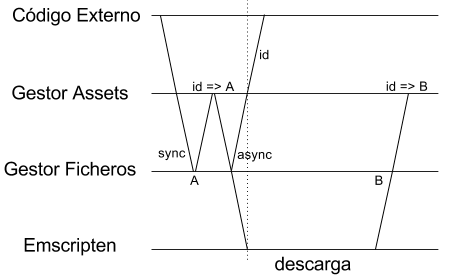
\includegraphics[width=0.80\linewidth]{async_file_manager}
    \caption{Esquema de la carga de ficheros.}
    \label{fig:async_file_manager}
\end{figure}
